\documentclass[9pt,twocolumn,twoside]{osajnl}
%% Select the journal you're submitting to
%% oe, boe, ome, osac, osajournal
\usepackage{cuted}
\usepackage{color, soul}
\journal{ao}
% Key:
% Express journals must have the correct journal selected:
% {oe} Optics Express
% {boe} Biomedical Optics Express
% {ome} Optical Material Express
% {osac} OSAC Continuum
% Other OSA journals may use:
% {osajournal} Applied Optics, Advances in Optics and Photonics, Journal of the Optical Society of America A/B, Optics Letters, Optica, Photonics Research

% Uncomment if submitting to Photonics Research.
% ONLY APPLICABLE FOR \journal{osajournal}
% \setprjcopyright

% Set the article type
%\articletype{Research Article}
% Note that article type is not required for Express journals (OE, BOE, OME and OSAC)
\setboolean{shortarticle}{false}

\title{A flexible, fast and benchmarked vectorial model for focused laser beams}
\author[1,*]{Qingfeng Li}
\author[1]{Maxime Chambonneau}
\author[1]{Markus Blothe}
\author[1,2]{Herbert Gross}
\author[1,2]{Stefan Nolte}

\affil[1]{Institute of Applied Physics, Abbe Ceter of Photonics, Friedirich-Schiller-University Jena, Albert-Einstein-Str. 15, 07745 Jena, Germany}

\affil[2]{Fraunhofer Institute for Applied Optics and Precision Engineering, Albert-Einstein-Str. 7, 07745 Jena, Germany}

\affil[*]{Corresponding author: qingfeng.li@uni-jena.de} %% email address is required

\begin{abstract}
	In-bulk processing of materials by ultrashort laser pulses has largely evolved over the last decade and still reveals new scientific and industrial potential. The development of any in-bulk processing application relies on the knowledge of laser propagation especially volumetric field distribution near the focus. Many commercial programs can simulate this, but, in order to adapt them, or to develop new methods, researchers need to create their own software. Besides, people also need to know the actually field distribution near the focus to evaluate their assumptions in the simulation. To help people easily get their access to these knowledges, we decided to release our high-precision field distribution measuring method as well as our in-house software InFocus \cite{InFocus} , under the Creative Commons 4.0 License, an open-source license. Our measurements provide 300-nm longitudinal resolution and diffraction limited lateral resolution. And the in-house software allows fast vectorial analysis of the focused volumetric field distribution in the bulk. It considered the lens induced spherical aberrations as well as the planar interface induced spherical aberrations. The simulations and measurements are systematically compared. 
\end{abstract}

\setboolean{displaycopyright}{true}

%%%%%%%%%%%%%%%%%%%%%%%%%%  body  %%%%%%%%%%%%%%%%%%%%%%%%%%
\begin{document}

\maketitle

\section{Introduction}\label{section:1}

Three-dimensional microprocessing of bandgap materials using ultrafast laser pulses has attracted intensive attention in wide range of areas related to academic research and industrial engineering in the last two decades. The nature of in-bulk processing allows many innovative applications include the fabrication of waveguides, gratings, binary data storage devices, channels and many other photonics devices \cite{Itoh2006, Gattass2008}. It has also been used for the new material processing procedures such as bonding \cite{Cvecek2019} and dicing \cite{Mishchik2017, Meyer2019} of bandgap materials. Among all the potential applications, the control of laser energy deposition is crucial. A large number of experimental and theoretical investigating of the ultrafast laser propagation and energy deposition has been intensively carried \cite{Couairon2007}. Depending on the optical power, the combined effects of diffraction, nonlinear refraction, nonlinear absorption and plasmas formation leads to large variety of spatial and temporal effects \cite{couairon2007femtosecond} ranging from self-focusing/defocusing self phase modulation to the formation of solitons \cite{stegeman1999optical}. In general, the description of the propagation of ultrashort laser pulses in bandgap material is given by the evolution of the optical field which follows the form of the scalar nonlinear Schr\"odinger equation  \cite{Sudrie2002}. Under this approximation, the laser beam is assumed remaining linearly polarized and the aberrations are often ignored. This assumption is valid when the laser is focused through a relatively low numerical aperature (NA < 0.6) into the low-refractive-index (< 1.5) materials with swallow depths (< 1-mm). However, when the laser is focused into the deep bulk of high-refractive-index material such as silicon, aberration induced by the interface must be considered. If high numerical aperature lens is used, polarization near the focus also turns to be complex. And in some cases, the focal lens would also introduced extra aberrations. In those conditions, using paraxial approximation would lead large deviation. 

In this paper, under the linear propagation condition, we are aiming to provide the electromagnetic (EM) field evolution by taking all the above mentioned extreme conditions into account. The results in this paper can easily adape to the nonlinear models and used as an initial condition for any nonlinear propagation investigating.  

One of the most widely used method for analysing the vectorial diffractions is the Debye-Wolf integral. As demonstrated by Leutenegger \emph{et~al.} \cite{leutenegger2006fast}, the 3D vectorial field distribution at the focus can be computed plane by plane under a proper transformation of the original Debye-Wolf integral. At a given axial position, the EM field in this plane is obtained by a two-dimensinal Fourier transform. Lin \emph{et~al.} \cite{Lin2012} have also demonstrated that this method is applicable to focusing through an interface between two mediums of mismatched refractive index. In this paper, we further adapt this method to non-aplanatic lens and provide a fast analysis tool which can evaluate the actual EM field distribution at the focus of those lens. Meanwhile, a non-destructive method is introduced to provide 300-nm longitudinal and diffraction limited lateral resolution measurements of the in-bulk volumetric intensity distribution. Our numerical and experimental methods benchmarked each other. 


\section{Methods} \label{section:2}
\subsection{3D-FT representation of the field vectors near the focus}
Using the form developed by Richards and Wolf \cite{richards1959electromagnetic}, the time-dependent field in the image regime of a system can be expressed by equation \eqref{eq:1}. $\textbf{e}$ and $\textbf{h}$ are the time-independent electric and magnetic vectors.

\begin{equation}\label{eq:1}
	\begin{aligned}
		\textbf{E}(x, y, z, t)&=\Re\{\textbf{e}(x, y, z)e^{-iwt}\},\\
		\textbf{H}(x, y, z, t)&=\Re\{\textbf{h}(x, y, z)e^{-iwt}\}.
	\end{aligned}	
\end{equation}

At any point $\textbf{P}(x,y,z)$ in the image space, the electric and magnetic vector express in the form as a summation of the plane waves that are leaving the aperture:

\begin{equation}
	\begin{aligned}\label{eq:2}
		\textbf{e}(x, y, z)&=-\frac{ik}{2\pi}\iint_\Omega\frac{\textbf{a}(s_x, s_y)}{s_z}e^{ik[\textbf{$\Phi$}(s_x, s_y)+s_xx+s_yy+s_zz]}\,ds_x\,ds_y,\\
		\textbf{h}(x, y, z)&=-\frac{ik}{2\pi}\iint_\Omega\frac{\textbf{b}(s_x, s_y)}{s_z}e^{ik[\textbf{$\Phi$}(s_x, s_y)+s_xx+s_yy+s_zz]}\,ds_x\,ds_y
	\end{aligned}
\end{equation}

where $\textbf{$\Phi$}(s_x, s_y)$ is the aberration function which describes the optical path difference between the aberrated and the spherical wavefront along $\textbf{s}$, $\textbf{a}$ and $\textbf{b}$ are the electric and magnetic strength vectors of the unperturbed electric and magnetic fields in the exit aperture, $k$ is the wave number, and $\Omega$ is the solid angle formed by all the geometrical optics ray. The phase factor shown in equation \eqref{eq:2} contains two parts, one is the scalar product of vector \textbf{s} and vector \textbf{r}$_p$, another is the vectorial aberration function. In this section henceforth we only discuss about the electric field since, apart from the strength vector, the two equations in \eqref{eq:2} are the same. 

Now lets consider a laser in-bulk focusing senario. As shown in Fig.~\ref{fig:1}, after the focusing lens it consist of materials 1 and 2 with refractive indices $n_1$ and $n_2$.

\begin{figure}
	\centering
	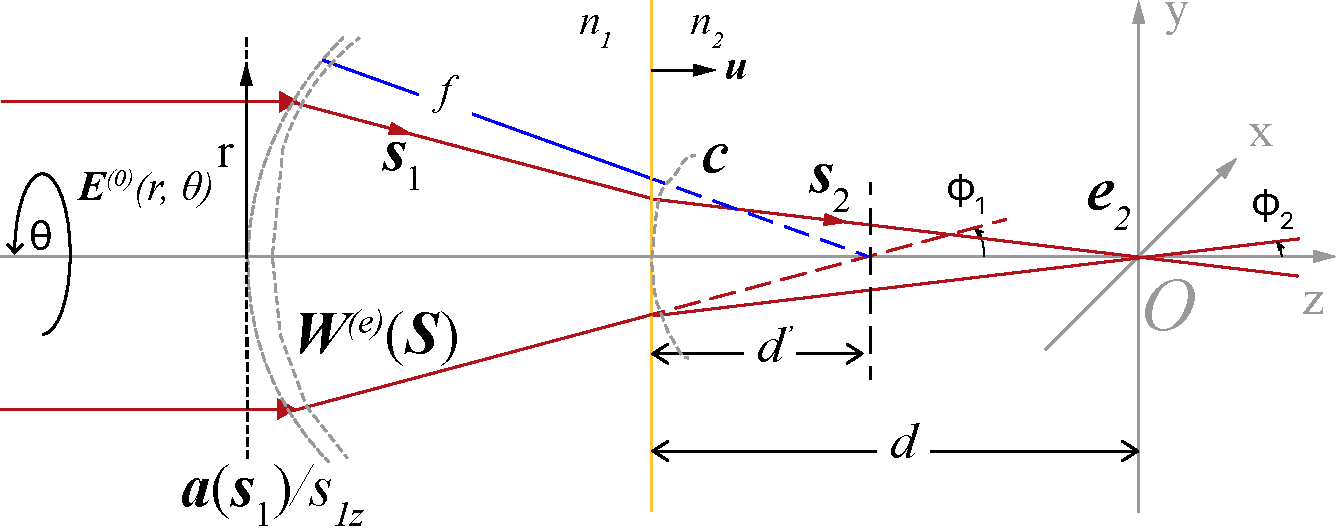
\includegraphics[width=\linewidth]{../AppOptics/figures/vectorDiffractionTheory.pdf}
	\caption{Diagram showing laser focused by a lens into two media seperated by a planar interface.}\label{fig:1}
\end{figure}

In material 1 and at the interface ($z=-d$), the electric field is given by

\begin{equation}\label{eq:3}
	\begin{aligned}
		\textbf{e}_1(x,y,-d)&=-\frac{ik_1}{2\pi}\iint_\Omega\textbf{C}(\vec{\mathbf{s}})\\
	&\times\exp[ik_1(s_{1x}x+s_{1y}y-s_{1z}d)]\,ds_{1x}\,ds_{1y}	
	\end{aligned}
\end{equation}
where 

\begin{equation}
	\textbf{C}^(\vec{\mathbf{s}})=\frac{\textbf{a}(s_{1x},s_{1y})e^{ik_1\Phi(s_{1x},s_{1y})}}{s_{1z}}
\end{equation}\label{eq:4}

by letting the strength vector $\mathbf{a}(s_{1x},s_{1y})$ absorb the aberration phase factor $e^{ik\Phi(\vec{\mathbf{s}})}$, the phase factor in \eqref{eq:3} contains only the scalar product of vector \textbf{s} and vector \textbf{r}$_p$. And the new strength vector $\textbf{C}(\vec{\mathbf{s}})$ is turned to be a complex strength vector.

\hl{Since there is no optical coating for all the cuboidal materials presented in this paper}, we assumed that each plane wave components refracting at the interface obeys the Fresnel's law. To determind the transmitted field in the second material, we also assumed that the field in the second material is constructed by the superposion of refracted plane waves. As the complex strength vector of the plane wave upon the interface is described as $\textbf{C}^(\vec{\textbf{s}})$, the strength vector of the transmitted plane wave can be described as a linear function of $\textbf{C}(\vec{\textbf{s}})$, i.e, $\textbf{T}\cdot\textbf{C}(\vec{\textbf{s}})$, where $\mathbf{T}$ is a refraction operator which is a function of angle of incident and $n_1$, $n_2$. Therefore, the transmitted field in the second material at the interface is given by 

\begin{equation}\label{eq:5}
	\begin{aligned}
		\textbf{e}_2(x,y,-d)&=-\frac{ik_1}{2\pi}\iint_{\Omega_1}\textbf{T}\cdot\textbf{C}(\vec{\textbf{S}})\\
		&\times\exp[ik_1(s_{1x}x+s_{1y}y-s_{1z}d)]\,ds_{1x}\,ds_{1y}		
	\end{aligned}
\end{equation}

On the other hand, we can also represent the field in the second material again as superposion of plane waves, which is a solution of time-dependent wave equation and can be written as

\begin{equation}\label{eq:6}
	\textbf{e}_2(\textbf{r}_p)=-\frac{ik_2}{2\pi}\iint_{\Omega_2}\textbf{F}(\vec{\mathbf{s}_2})\exp(ik_2\vec{\textbf{s}}_2\cdot\mathbf{r}_p)\,ds_{2x}\,ds_{2y}.
\end{equation}

One can notice that \eqref{eq:5} is the boundary condition of \eqref{eq:6}. Now let's establish the relation between $\vec{\textbf{s}_1}$ and $\vec{\textbf{s}_2}$.

According to the law of refraction,

\begin{equation}\label{eq:7}
	k_1(\vec{\textbf{u}}\times\vec{\textbf{s}_1})=k_2(\vec{\textbf{u}}\times\vec{\textbf{s}_2}),
\end{equation}
where $\vec{\textbf{u}}$ is the unit vector that normal to the interface. When a planar interface is presented $\vec{\textbf{u}}=(0,0,1)$, and we have
\begin{equation}\label{eq:8}
	k_1s_{1x}=k_2s_{2x},\,\,\,\,
	k_1s_{1y}=k_2s_{2y}.
\end{equation} 

By taking the coordinate transformation, equation \eqref{eq:6} yields

\begin{equation}\label{eq:9}
	\begin{aligned}
		\mathbf{e}_2(\mathbf{r}_p)&=-\frac{ik_2}{2\pi}\iint_{\Omega_1}\mathbf{F}(\vec{\mathbf{s}_2})\\
		&\times\exp(ik_2\vec{\mathbf{s}_2}\cdot\vec{\mathbf{r}_p})\mathbf{J}_0(s_{1x},s_{1y};s_{2x},s_{2y})\,ds_{1x}\,ds_{1y},		
	\end{aligned}
\end{equation}

where $\mathbf{J}_0$ is the Jacobian of the coordinate transformation obtained from equation \eqref{eq:8}:

\begin{equation}\label{eq:10}
	\mathbf{J}_0=(\frac{k_1}{k_2})^2,
\end{equation}
As equation \eqref{eq:9} must satisfies the boundary condition represented by equation \eqref{eq:5}, we have
\begin{equation}\label{eq:11}
	\mathbf{F}(\vec{\mathbf{s}_1},\vec{\mathbf{s}_2})=(\frac{k_2}{k_1})\mathbf{T}\cdot\mathbf{C}(\vec{\mathbf{s}})\exp[id(k_2s_{2z}-k_1s_{1z})].
\end{equation}

By substituting into equation \eqref{eq:9} we obtain the electric field in the second material:

\begin{equation}
	\begin{aligned}\label{eq:12}
	\mathbf{e}_2(x,y,z)&=-\frac{ik^2_2}{2\pi k_1}\iint_{\Omega_1}\mathbf{T}\cdot\mathbf{C}(\vec{\mathbf{s}})\\
	&\times\exp[id(k_2s_{2z}-k_1s_{1z})]\exp(ik_2s_{2z}z)\\
	&\times\exp[ik_1(s_{1x}x+s_{1y}y)]\,ds_{1x}\,ds_{1y}.
	\end{aligned}
\end{equation}

The first phase factor $\exp[id(k_2s_{2z}-k_1s_{1z})]$ stands for the aberration induced by the interface. The second phase factor $\exp(ik_2s_{2z}z)$ accounts for the phase accumulation when propagating along the z-axis, whereas the third term $\exp[ik_1(s_{1x}x+s_{1y}y)]$ represents the phase difference of the wave front at off-axis points (x,y,z) with respect to the on-axis point (0,0,z).

Depends on the coordinate one has choosen, the following forms of the wave vectors are equivalent:

\begin{equation}\label{eq:13}
	\begin{aligned}
		&\vec{k_1}=\begin{pmatrix}
			k_{1x}\\
			k_{1y}\\
			k_{1z}
		\end{pmatrix}=k_1	
		\begin{pmatrix}
			-s_{1x}\\
			-s_{1y}\\
			s_{1z}	
		\end{pmatrix}=k_1
		\begin{pmatrix}
			-\sin\phi_1\cos\theta\\
			-\sin\phi_1\sin\theta\\
			\cos\phi_1	
		\end{pmatrix},\,\,\\\\
	&\vec{k_2}=\begin{pmatrix}
		k_{2x}\\
		k_{2y}\\
		k_{2z}
	\end{pmatrix}=k_2	
		\begin{pmatrix}
			-s_{2x}\\
			-s_{2y}\\
			s_{2z}	
		\end{pmatrix}=k_2
		\begin{pmatrix}
			-\sin\phi_2\sin\theta\\
			-\sin\phi_2\cos\theta\\
			\cos\phi_2	
		\end{pmatrix}.		
	\end{aligned}
\end{equation}

Therefore, $\,ds_{1x}\,ds_{1y}$ can be written as $\,dk_{1x}\,dk_{1y}/k_1^2$ and the interface induced aberration can be written as 
\begin{equation}\label{eq:14}
	\Psi(\phi_1,\phi_2,d)=d(n_2\cos\phi_2-n_1\cos\phi_1).
\end{equation}
The spherical-polar form of the complex strength vector after the interface is
\begin{equation}\label{eq:15}
	\mathbf{C}(\phi_1,\phi_2,r,\theta)=\mathbf{T}(\phi_1,\phi_2,\theta)\cdot\mathbf{a}(r,\theta)e^{ik_1\Phi(r,\theta)}/\cos\phi_1.
\end{equation}
By using $\mathbf{c}(\phi_1,\phi_2,r,\theta)$ to brief note $\mathbf{T}(\phi_1,\phi_2,\theta)\cdot\mathbf{a}(r,\theta)e^{ik_1\Phi(r,\theta)}$, \eqref{eq:12} can be finally rewritten as

\begin{equation}
	\begin{aligned}\label{eq:16}
		\mathbf{e}_2(x,y,z,d)&=-\frac{ik^2_2}{2\pi k^3_1}
		\iint_{r<R}[\mathbf{c}(\phi_1,\phi_2,\theta)e^{ik_0\Psi(\phi_1,\phi_2,d)}e^{ik_{2z}z}/\cos\phi_1]\\
		&\times \exp[-i(k_{1x}x+k_{1y}y)]\,dk_{1x}\,dk_{1y}.
	\end{aligned}
\end{equation}

By using Leutenegger's method \cite{leutenegger2006fast}, setting $|\mathbf{c}|=0$ when $r>R$, the Debye-Wolf intergral is now expressed as the Fourier transform of the field distribution after the interface formed by the two material. And finally result in

\begin{equation}\label{eq:17}
	\mathbf{e}_2(x,y,z,d)=-\frac{ik^2_2}{2\pi k^3_1}\mathcal{F}[\mathbf{c}(\phi_1,\phi_2,\theta)e^{ik_0\Psi(\phi_1,\phi_2,d)}e^{ik_{2z}z}/\cos\phi_1].
\end{equation}

As inspired by Leutenegger \cite{leutenegger2006fast}, we used the chirped Z-transform (CZT) algorithm \cite{Bakx2002} for the Fourier transformation. With this algorithm, it (a) allows breaking the relationship between the sampling points (M) over the aperture radius and the minimal sampling points (N) for fast Fourier transform (FFT), (b) allows an implicit frequency offset, and (c) internalizes the zero padding. Applying this generalization, one can adapt the sampling step in the focus field independently of the sampling step in the input field, introduce an additional shift of the region of interest, and finally improve the computational efficiency.

% The Jacobian of the transformation to spherical polar coordinate is 
% \begin{equation}\label{eq:17}
% 	\mathbf{J}_p=\sin\phi_1\cos\phi_2;
% \end{equation}
% therefore
% \begin{equation}\label{eq:18}
% 	ds_{1x}ds_{1y}=\sin\phi_1\cos\phi_1d\phi_1d\theta.
% \end{equation}
% and equation \eqref{eq:12} expressed as
% \begin{equation}
% 	\begin{aligned}\label{eq:19}
% 	\mathbf{e}_2(\mathbf{r}_p,d)&=-\frac{ik_1}{2\pi}\iint_{\Omega_1}\frac{\mathbf{c}(\phi_1,\phi_2,\theta)}{\cos\phi_1}\cos\phi_1\\
% 	&\times\exp[ik_0d(n_2\cos\phi_2-n_1\cos\phi_1)]\\
% 	&\times\exp\{ik_2r_p[\sin\phi_2\sin\phi_p\cos(\theta-\theta_p)+\cos\phi_2\cos\phi_p]\}\sin\phi_2d\phi_2d\theta.
% 	\end{aligned}
% \end{equation}
% Let's define that 
% \begin{equation}\label{eq:20}
% 	\Psi(\phi_1,\phi_2,d)=d(n_2\cos\phi_2-n_1\cos\phi_1),
% \end{equation}
% and 
% \begin{equation}\label{eq:21}
% 	\mathbf{C}(\phi_1,\phi_2,\theta)=\mathbf{c}(\phi_1,\phi_2,\theta)\delta(\rho-k_1),	
% \end{equation}
% equation \eqref{eq:19} can be written as the following triple integral
% \begin{equation}
% 	\begin{aligned}\label{eq:22}
% 		\mathbf{e}_2(\mathbf{r}_p,d)&=-\frac{i}{2\pi k_1}\\
% 		&\times\int^{2\pi}_0\int^\pi_0\int^\infty_0[\mathbf{C}(\phi_1,\phi_2,\theta)\Psi(\phi_1,\phi_2,d)]\\
% 		&\times\exp\{ik_2r_p[\sin\phi_2\sin\phi_p\cos(\theta-\theta_p)+\cos\phi_2\cos\phi_p]\}\rho^2\sin\phi_2\,d\phi_2\,d\theta\,d\rho.
% 	\end{aligned}		
% \end{equation}
% According to McCutchen's method \cite{McCutchen:64} equation \eqref{eq:22} is the three-dimensional Fourier transform (3D-FT) of $[\mathbf{C}(\phi_1,\phi_2,\theta)\Psi(\phi_1,\phi_2,d)]$. In other words, explicitly driven from Debye-Wolf intergral, the transmitted field in the second material is the 3D-FT of the product of strength vector after the interface and an aberration function. In practise, after transformation to Cartesian coordinate, using FFT algorithm can result in an output plane with the same transverse dimension and sampling size as the aperture. By using Leutenegger's method, 
% \begin{equation}
% 	\mathbf{e}_2(x,y,z,d)=-
% \end{equation}
\subsection{Representation of the complex strength vector}
To determind the complex strength vector $\mathbf{c}$, let's assume that a linear polarized wave incident upon a lens. By choosing the corresponding Cartesian coordinate and letting the y and z-component of the incident electric field as zero, the incident electric strength vector can be written as

\begin{equation}\label{eq:18}
	\mathbf{E}^{(0)}=
	\begin{pmatrix}
		E_0\\
		0\\
		0
	\end{pmatrix}.
\end{equation}

According to T\"or\"ok \emph{et~al.} \cite{torok1995electromagnetic}, the transform relation betweeen the incident vector and the refracted vector after the interface can be expressed by a refraction operator $\mathbf{T}$. This operator has a matrix form of 

\begin{strip}
	\begin{equation}\label{eq:19}
		\mathbf{T}=A(\phi_1)
		\begin{bmatrix}
			\tau_p\cos^2\theta\cos\phi_2+\tau_s\sin^2\theta& (\tau_p\cos\phi_2-\tau_s)\cos\theta\sin\theta& \tau_p\cos\theta\sin\phi_2\\
			(\tau_p\cos\theta-\tau_s)\cos\theta\sin\theta& \tau_s\cos^2\theta+\tau_p\cos\phi_2\sin^2\theta& \tau_p\sin\theta\sin\phi_2\\
			-\tau_p\cos\theta\sin\phi_2& -\tau_p\sin\theta\sin\phi_2& \tau_p\cos\phi_2
		\end{bmatrix}.
	\end{equation}	
\end{strip} 

Here $\tau_s$ and $\tau_p$ are the Fresnel transmission coefficients for s-polarized and p-polarized light, respectively. The function $A(\phi_1)$ is an apodization function that depends on the lens. And when the system obeys Abbe's sine condition, i.e, is aplanatic, then
\begin{equation}\label{eq:20}
	A(\phi_1)=f l_0\sqrt{\cos\phi_1}
\end{equation}
where $f_0$ is the focal length of the lens in vacuum and $l_0$ is an amplitude factor. \hl{It is worth noting that, since the complex strength vector has absorb the aberration phase factor, even many non-aplanatic lens are discussed in this paper, the Abbe's sine condition is still valid in this step.} 

To represent the aberration phase factor and to scale it in the scale of wavelength $\lambda$, the aberration factor $e^{ik_1\Phi(r,\theta)}$ is rewritten as $e^{i2\pi W(r,\theta)}$. To describe a circular lens induced wavefront aberration and calculate the deviation of the wavefront to an ideal spherical shape, one widely used method is to represent it by Zernike polynomials.  %In this paper, we use the notation convention defined by R. Noll \cite{Noll1976}.
% For spherical lens, the primary aberrations can be represented by the Seidel formula. The aberration function $W$ can be written as:
% \begin{equation}\label{eq:21}
% 	\begin{aligned}
% 	W&=W_{040}r^4+W_{131}yr^3\cos\theta_0+W_{222}y^2r^2\cos^2\theta_0\\
% 	&+W_{220}y^2r^2+W_{311}y^3r\cos\theta_0
% 	\end{aligned}
% \end{equation}
% where $W_{040}$ and so on are the Seidel coefficients, $r$ is the normalized aperature radius on the entrence pupil plane, $y$ is the field height and $\theta_0$ is the pupil azimuth angle. It is worth to note that, in Seidel aberration, only primary aberration is considered. And for most of the in-bulk laser processing condition, the laser beam is normal incident to the lens, and the chief ray is along the optical axis. Therefore, only the on-axis spherical aberration play significant role and the off-axis aberration can be ignored. The aberration function can be simplified as 
% \begin{equation}\label{eq:22}
% 	W=W_{040}r^4.
% \end{equation}

By using the vendors provided lens data, the aberration function can be calculated in the form of superposion of Zernike polynomials through any home made ray tracing program or commercial softwares such as Zemax or Code V. In this paper, we used Zemax to calculate the aberration function and used the notation convention defined by R. Noll \cite{Noll1976} (so called Zernike standard polynomials):
\begin{equation}\label{eq:22b}
	W = \sum_{i=1}^{37}c_iZ_i(r,\theta_0),
\end{equation}
where $c_i$ is the orthonormal Zernike coeffient computed by Zemax, $Z_i$ is the corresponding Zernike standard polynomial.

Finally from equations \eqref{eq:15} and \eqref{eq:18}-\eqref{eq:22b}, the complex strength vector after the interface can be written as:

\begin{strip}
	\begin{equation}
		\begin{aligned}\label{eq:23}
			\mathbf{c}&=f l_0\sqrt{\cos\phi_1}\\
			&\times\begin{bmatrix}
				\tau_p\cos^2\theta\cos\phi_2+\tau_s\sin^2\theta& (\tau_p\cos\phi_2-\tau_s)\cos\theta\sin\theta& \tau_p\cos\theta\sin\phi_2\\
				(\tau_p\cos\theta-\tau_s)\cos\theta\sin\theta& \tau_s\cos^2\theta+\tau_p\cos\phi_2\sin^2\theta& \tau_p\sin\theta\sin\phi_2\\
				-\tau_p\cos\theta\sin\phi_2& -\tau_p\sin\theta\sin\phi_2& \tau_p\cos\phi_2
				\end{bmatrix}
				\begin{bmatrix}
					e^{i2\pi W}&0&0\\
					0&e^{i2\pi W}&0\\
					0&0&e^{i2\pi W}
				\end{bmatrix}
				\begin{bmatrix}
					E_0\\
					0\\
					0
				\end{bmatrix}.
		\end{aligned}
	\end{equation}	
\end{strip}

By substituting \eqref{eq:23} into \eqref{eq:12}, a CZT algorism based highly-efficient propagation model is compelete, it allows fast in-focus fields calculation by taking both lens-induced and interface-induced aberration into account.

\subsection{In-bulk propagation imaging}
To have a systematic comparison with the numerical results. We intruduced the non-destructive measurements on the in-bulk volumetric intensity distributions, which rely on (i) the focusing of the laser beam at the exit surface of the sample with desired thickness, and (ii) an inverted microscope working in transmission for imaging the beam profile in the xy plane for various positions of the focusing objective along z. The experimental set-up is schematically depicted in Fig.~\ref{fig:2}.
\begin{figure}
	\centering
	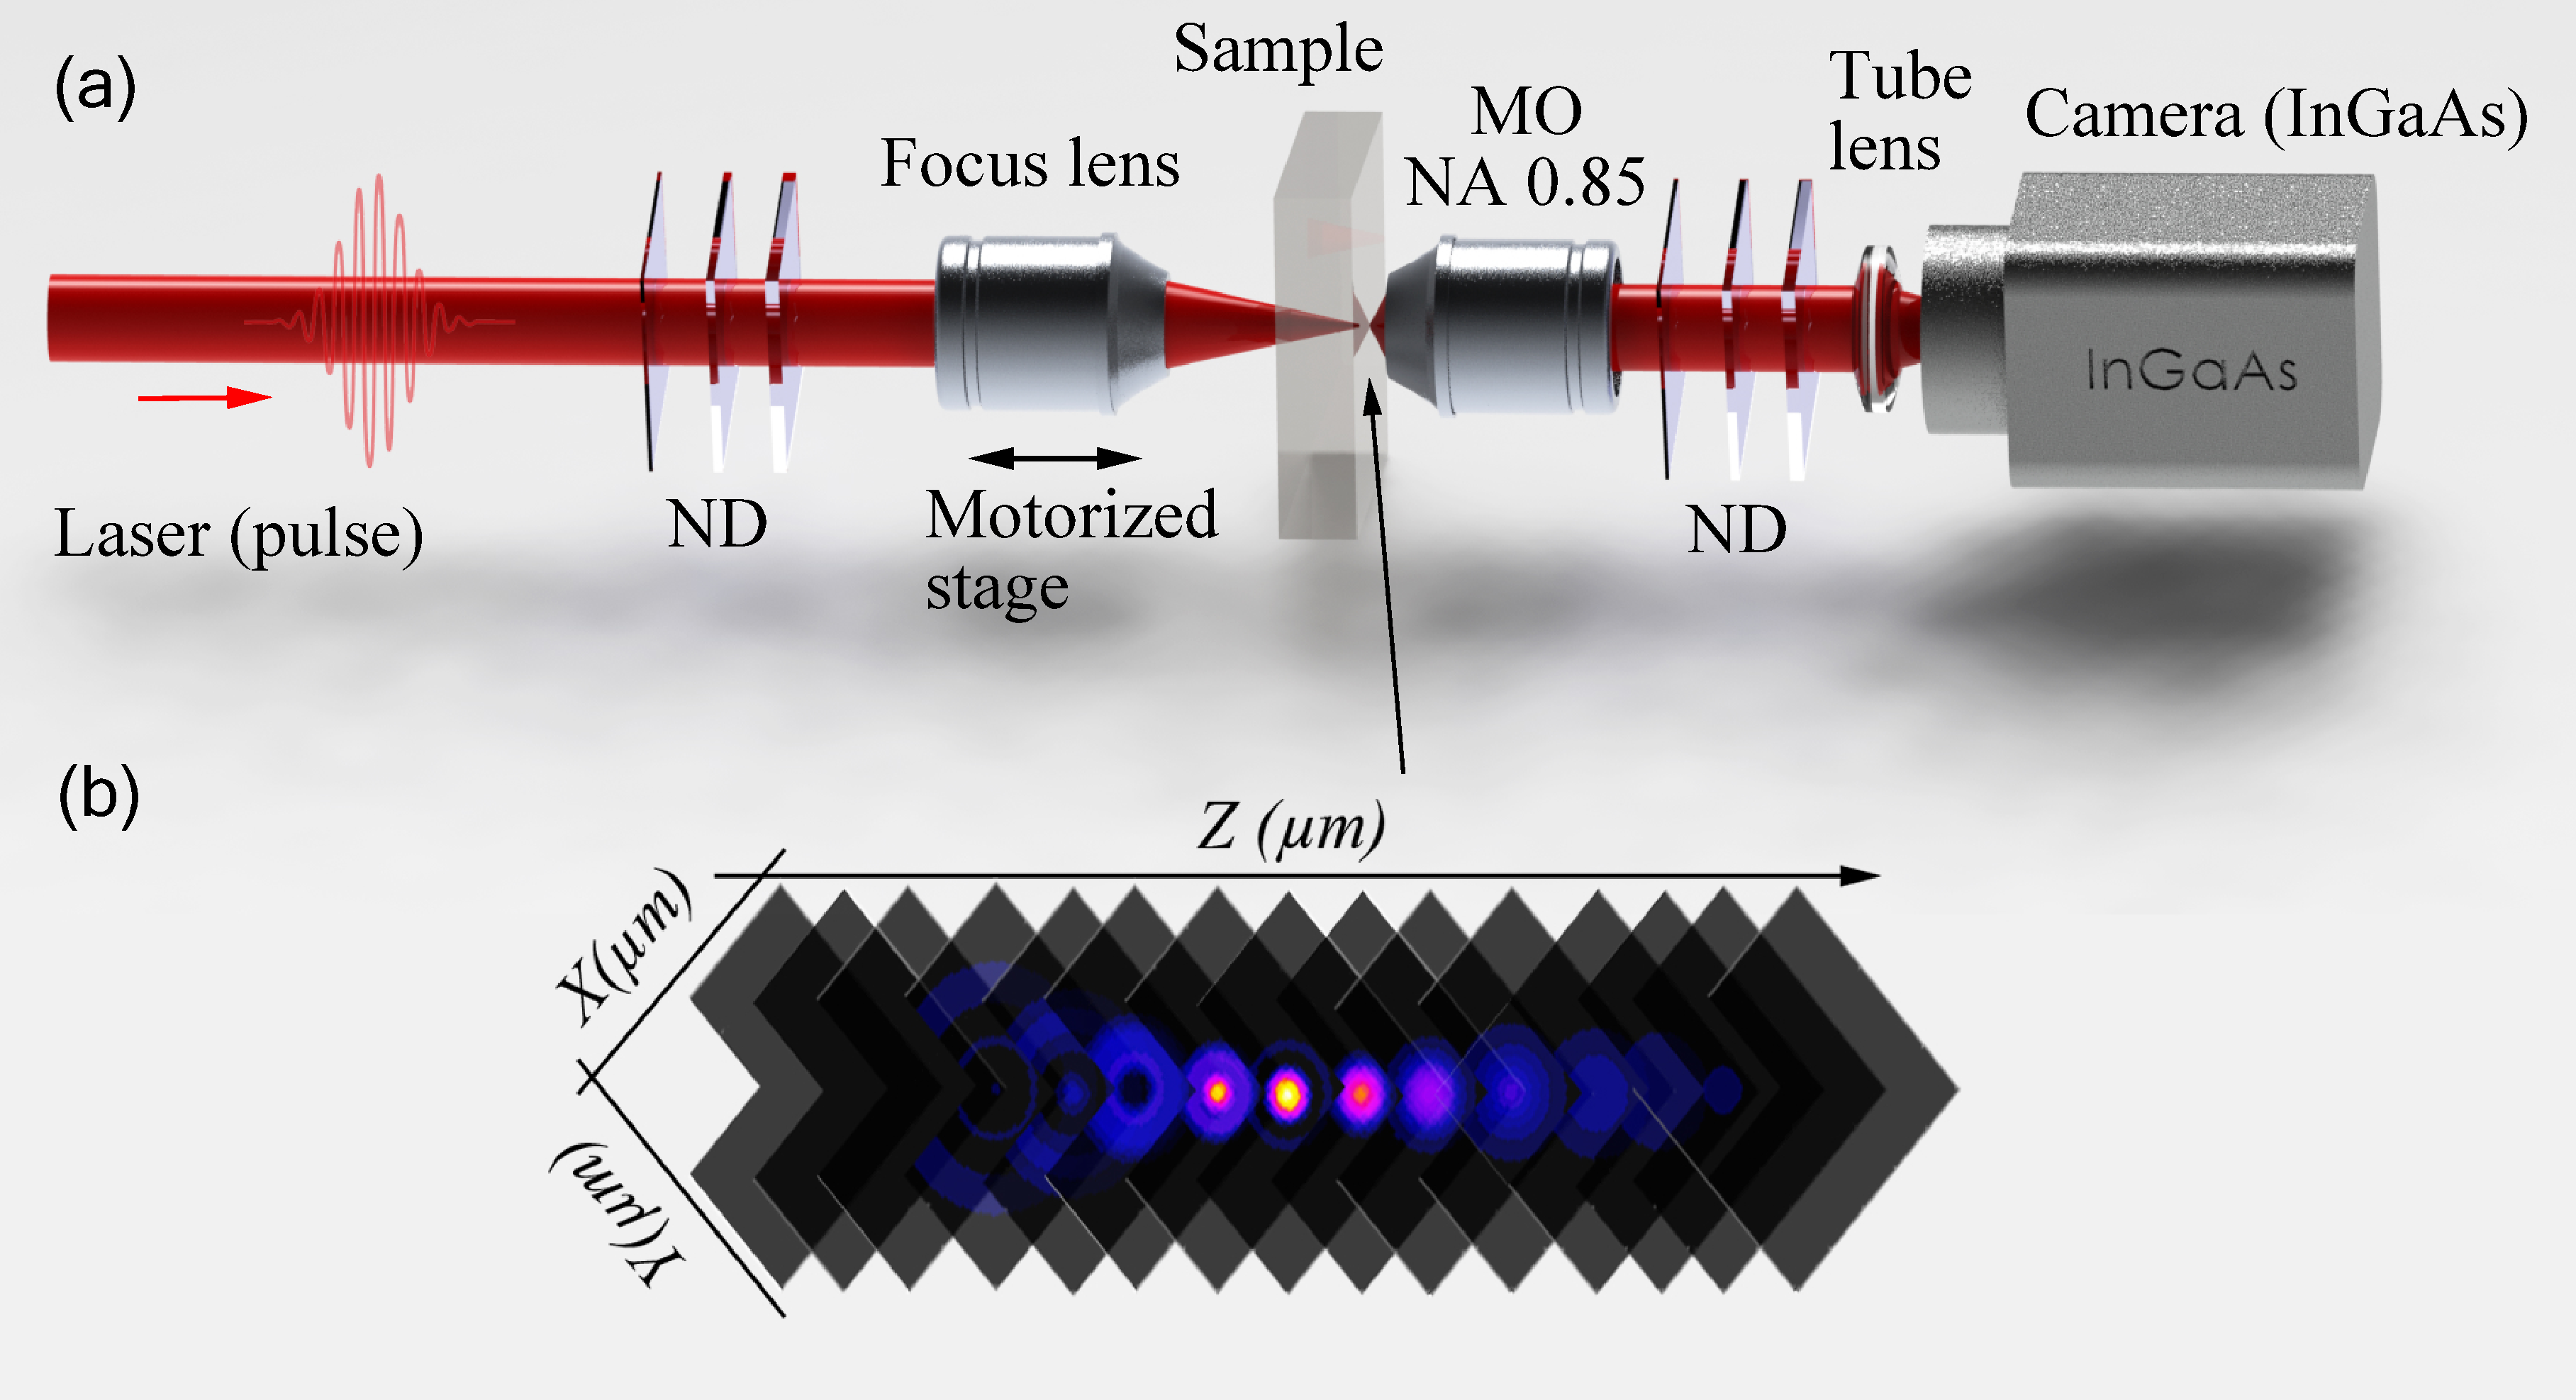
\includegraphics[width=\linewidth]{../AppOptics/figures/setup.pdf}
	\caption{Illustration of in-bulk propagation imaging processes. (a) Experimental setup, MO: microscope objective lens, ND: neutral density filters. (b) Intensity distribution near the focal region reconstructed from the stacking of captured images applying a z-scan.}\label{fig:2}
\end{figure}

The measurements can explicitly devide into two steps. The first step consist in focusing the laser beam with identical characterisitics (beam size, spectrum, phase distribution, etc.) as the simulation. Before focusing, the pulse energy is kept as low as possible (typically, on the order of 18~pJ) for avoiding nonlinear propagation. In this case, we can set the maximum fluence position as the reference and overlap it with the exit surface of the cuboidal sample. The second step consists in imaging the exit surface of the sample with the inverted microscope working in transmission along the z axis. This microscope is composed of an collecting infinity-corrected objective lens whose numerical aperature (NA) is larger than the focusing one, a tube lens and an InGaAs array (Xenics, Bobcat 320). In this paper, the NA of the imaging objective lens is kept as 0.85 and its focal plane is precisely adjusted at the exit surface of the sample under the white light illumincation thanks to a precision stage (Physik Instrumente, M-126DG1). When there is no sample (focus in air), this plane can be arbitrarily choosen. The fluence evolution along the z-axis is recorded by alternating 100-nm movements of the focus lens (corresponding to $n\times100$-nm displacement in a sample with refractive index of $n$), and image acquisitions by the camera. The stack of images is then post-processed for reconstructing the fluence distribution as follows. Firstly, due to the jitter of the laser, some of the recorded images may show a much higher maximum intensity compare to both the preceding and the following one. These rare outlier images are replaced by the average of the preceding and the following images. Then, in the corner of each image, the noise is calculated as the average of the pixel amplitude, and subsequently subtracted to all pixels. The image containing the maximum grey level is found for a normalization of the whole stack. Two images before and after this latter image are defined for evaluating and correcting the residual tilt of the collecting objective lens with respect to the incoming beam. Finally, the beam propagation is reconstructed by displaying a cross section (along x or y) of each image at the center of the beam. 

\section{Results and discussions} \label{section:3}
Based on the vectorial analysing model and the measurements setup, we selected four typical senarios, i.e. Gaussian beam focused by a plano-convex lens, Gaussian beam focused by an aspherical lens in air, exotic beams focused by objective lens in air, and finally Gaussian beam focused into a bulk material by objective lens for the demonstrations. The vendors of the lens and other information of those four senarios are list in table \ref{tab:1}.
\begin{table*}
	\centering
	\begin{tabular}[c]{|l|c|c|c|c|c|c|}
		\hline
		\rowcolor{gray}
		Section, Vendor, Lens& f [mm]& NA & $\Phi$ [mm] & $\omega$ [mm] & $\lambda$ [nm]&n$_2$ \\
		\hline
		3.A, Thorlabs, LA1951-C & 25.3 & - & 25.4 & Gaussian 5.2 & 1555 & 1 \\
		\rowcolor{lightgray}
		3.B, Thorlabs, C240TME-C & 8.0 & 0.50 & 8.0 & Gaussian 5.2 & 1555 & 1\\
		3.C, Mitutoyo, 20$\times$ Plan Apo NIR & 10.0 & 0.4 & 8 & user define & 1030 & 1\\
		\rowcolor{lightgray}
		3.C, Mitutoyo, 50$\times$ Plan Apo NIR HR & 4.0 & 0.65 & 5.2 & Gaussian 5.2 & 1555 & 3.475\\
		\hline
	\end{tabular}	
	\caption{Prescription data of the lens for the demonstrations. f is the focal length, NA is the numerical aperture, $\Phi$ is the entrence aperture diameter, $\omega$ is the incident beam waist, $\lambda$ is the central wavelength of the incident beam and $n_2$ is the refractive index of the focused-in medium.}\label{tab:1}
\end{table*}

\subsection{Gaussian beam focused by plano-convex lens in air}
The plano-convex lens is one of the most simple coverging lens that has been widely used to focus collimated light. However, even the asymmetry design can minimizes the spherical aberration by letting the curved surface face towards the collimated beam, it cannot be completely reduced. In our first demonstration, we chose a plano-convex lens (Thorlabs LA1951-C) and used the two methods mentioned in section \ref{section:2} to evaluate the intensity distribution at its focus. The experimental condition is briefly described in Tab.\ref{tab:1} (3.A), a collimated laser beam with incident beam waist (1/$e^2$) of 5.2-mm and wavelength of 1555-nm is focused by the lens in air. To calculate the lens induced aberrations, in Zemax the aperature type is set as 'Entrance Pupil Diameter' and its valus is set as 10.4-mm. \hl{The apodization factor $G$ (refers to the rate of decrease of the beam amplitude as a function of radial pupil coordinate) is set as 1. The beam amplitude is normalized to unity at the center of the pupil, and the amplitude at other points in the entrance pupil is given by $A(\rho)=e^{-G\rho^2}$, where $\rho$ is the normalized pupil coordinate.} Under this approximation, the aberration induced by the lens is calculated and represented by the standard zernike coefficients. In Tab.~\ref{tab:2} the nonzero coefficients are listed upto term 37. Finally, the normalized intensity distribution near the focus can be calculated based on equations \eqref{eq:17} and \eqref{eq:23}. 
\begin{table}
	\centering
	\begin{tabular}[c]{|l|c|c|}
		\hline
		\rowcolor{lightgray}
		$Z_1$ & 2.484 & 1 \\
		$Z_4$ & 2.171 & $\sqrt{3}(2r^2-1)$ \\
		\rowcolor{lightgray}
		$Z_{11}$ & 0.581 & $\sqrt{5}(6r^4-6r^2+1)$ \\
		$Z_{22}$ & 0.009 & $\sqrt{7}(20r^6-30r^4+12r^2-1)$\\
		\rowcolor{lightgray}
		$z_{37}$ & 0.0002 & $\sqrt{9}(70r^8-140r^6+90r^4-20r^2+1)$\\
		\hline
	\end{tabular}	
	\caption{Nonzero terms of the Zernike standard coefficients calculated at the exit pupil of the plano-convex lens Thorlabs LA1951-C.}\label{tab:2}
\end{table}

As shown in Fig.~\ref{fig:3}, when beam propagated from the left to the right and be focused by the plano-convex lens LA1951-C under the normal incident condition, the experimental and the simulated results are systematically compared. Fig.~\ref{fig:3} (a) (c) show the normalized longitudinal intensity distributions and Fig.~\ref{fig:3} (b) (d) show the intensity distribution at the focal plane. To quantitatively evaluate the goodness of fit, in Fig.~\ref{fig:3} (e-f), \hl{we plot the normalized intensity value along the x and y central segment at the focal plane. Meanwhile, the square of the experiment to simulation differences are also point-by-point plotted along the same axis. Finally the root-mean-square deviation (RMSD) of the two types of results are calculated to have an overall evaluation of the difference.}

As shown in Fig.~\ref{fig:3} (e), along the x-axis, the experimental beam wasit at $1/e^2$ is measured as 10.6~$\mu$m and the simulated one is 11.4~$\mu$m. The RMSD of the two profiles is 0.051. Similar comparisons are applied to the profiles along the y-axis. The experimental beam wasit is measured as 11.3~$\mu$m, the simulated one is 11.4~$\mu$m and the RMSD is 0.046. From the quantitative comparison one can notice that, deviating from the simulated results, the experimental one exhibits the feature of ellipticity. This deviation is most probably due to the fact that the during the simulation the incident beam has been oversimplified as a circular gaussian beam. Except of that, the simulated results fit well with the experimentent. 

Due to the misalignment of the images stacking, we could not provide the RMSD of the longitudinal intensities. However, the overview of the longitudinal intensity distributions through the focal regime shown in Fig.~\ref{fig:3} (a) (c) indicate simular positive spherical aberration features. The twisted tail on the left hand side of Fig.~\ref{fig:3} (a) is most probably caused by the difficulty of finding the image center during the post-processing. Except of that, the aberration features as well as the overall lengths of the focal regime are identical.

\begin{figure}
	\centering
	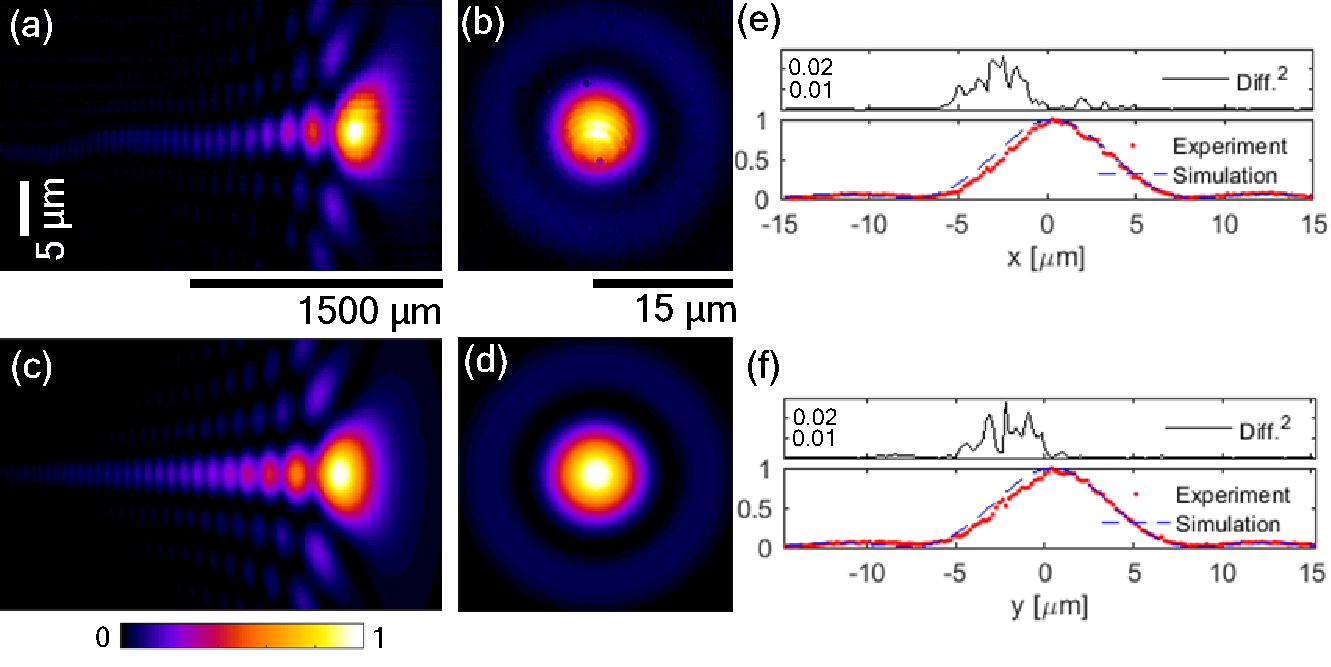
\includegraphics[width=\linewidth]{../AppOptics/figures/LA1951air.pdf}
	\caption{Intensity distribution near the focus of a plano-convex lens (LA1951-C) in air with a gaussian beam as the input. (a) Experimentally measured intensity along x-z plane; (b) experimentally measured intensity at the focal plane; (c) simulated intensity along x-z plane; (d) simulated intensity at the focal plane. And intensity profiles comparisons at the focal plane (e) along the x-axis; (f) along the y-axis.}\label{fig:3}
\end{figure}



\subsection{Gaussian beam focused by aspheric lens in air}
In order to achieve in-bulk processing, tightly focused laser beams are sometimes required. To achieve the diffraction-limited high quality tight focusing, a cost-efficient single element solution is to use an aspheric lens. It worth to noting that a single aspheric lens is also not aplanatic, and the higher order aberrations should be considered.
%the converging waves after the exit pupil are not fit to the spherical wave approximation used in Debye-Wolf integral. Even this deviation can be ignored under the conditions when a collimated light is normally incident to a low NA lens, extra caution should be taken when the appling conditions varied.} 
In this paper, a Thorlabs C240TME-C aspheric lens with NA equals to 0.5 is used for the demonstration.According to design file provided by the vendor. \hl{As the input beam waist radius is 5.2-mm which has overfilled the entrance pupil of the lens by a factor of 1.3, the apodization factor $G$ (refers to the rate of decrease of the beam amplitude as a function of radial pupil coordinate) is set as $\sqrt{1/1.3}$, i.e. 0.877. And the beam amplitude is normalized to unity at the center of the pupil. The amplitude at other points in the entrance pupil is given by $A(\rho)=e^{-G\rho^2}$, where $\rho$ is the normalized pupil coordinate.} Under this approximation, the aberration induced by the lens is calculated and represented by the standard zernike coefficients. In Tab. \ref{tab:3} the nonzero coefficients are listed upto term 37. For the simplicity, we first dedicate to the in-air focus condition. Therefore, the refractive index $n_2$ of the medium after the lens is 1. And the normalized intensity distribution near the focus can be calculated based on \eqref{eq:17} and \eqref{eq:23}. 
\begin{table}
	\centering
	\begin{tabular}[c]{|l|c|c|}
		\hline
		\rowcolor{lightgray}
		$Z_1$ & 0.5821 & 1 \\
		$Z_4$ & 0.3187 & $\sqrt{3}(2r^2-1)$ \\
		\rowcolor{lightgray}
		$Z_{11}$ & -0.0209 & $\sqrt{5}(6r^4-6r^2+1)$ \\
		$Z_{22}$ & -0.007 & $\sqrt{7}(20r^6-30r^4+12r^2-1)$\\
		\rowcolor{lightgray}
		$z_{37}$ & -0.007 & $\sqrt{9}(70r^8-140r^6+90r^4-20r^2+1)$\\
		\hline
	\end{tabular}	
	\caption{Nonzero terms of the Zernike standard coefficients calculated at the exit pupil of the aspherical lens Thorlabs C240TME-C.}\label{tab:3}
\end{table}

As shown in Fig.~\ref{fig:3b}, when a collimated laser beam with wavelength of 1555-nm and beam waist of 5.2-$\mu$m propagated from the left to the right and be focused by the aspherical lens C240TME-C under the normal incident condition, the experimental and the simulated results are systematically compared. Fig.~\ref{fig:3b} (a) (c) shown the normalized longitudinal intensity distributions and Fig.~\ref{fig:3b} (b) (d) shown the intensity distribution at the focal plane. The overall distributions are very similar. To quantitatively evaluate how good the simulation results fit with the experimental one, in Fig.~\ref{fig:3b} (e-g) the experimental intensity profiles are plot against the simulated one. Meanwhile, the square of the experiment to simulation differences are also point-by-point plotted along each axis. Finally, the root-mean-square deviation (RMSD) of the two results are calculated for each axis. As shown in Fig.~\ref{fig:3b} (e), by setting the intensity maximized position as the origin, along x-axis the intensity profiles and the square of their differences are plot from  -5~$\mu$m to 5~$\mu$m. The experimental beam waist is measured as 2.64~$\mu$m, the simulated one is 2.93~$\mu$m and the RMSD of the normalized intensity is 0.0305. As shown in Fig.~\ref{fig:3b} (f), similar comparisons are applied to the profile along y-axis, in which the experimental beam waist is 2.65~$\mu$m, the simulated one is 2.73~$\mu$m and the RMSD is 0.0326. A further comparison of applied to the profiles along z-axis, the RMSD of the normalized longitudinal profiles is 0.0322. To anchor a reference, we also simulated the intensity distribution near the focus without considering the influence of the aberration. In this case, the RMSD of the normalized profiles along x, y, z-axis are 0.0382, 0.0359 and 0.0365. In another words, by taking the aberration induced by the C240TME-C lens into account, the RMSDs have decreased by 20.2\%, 9.2\% and 11.8\% along x, y and z-axis correspondingly.

\begin{figure}
	\centering
	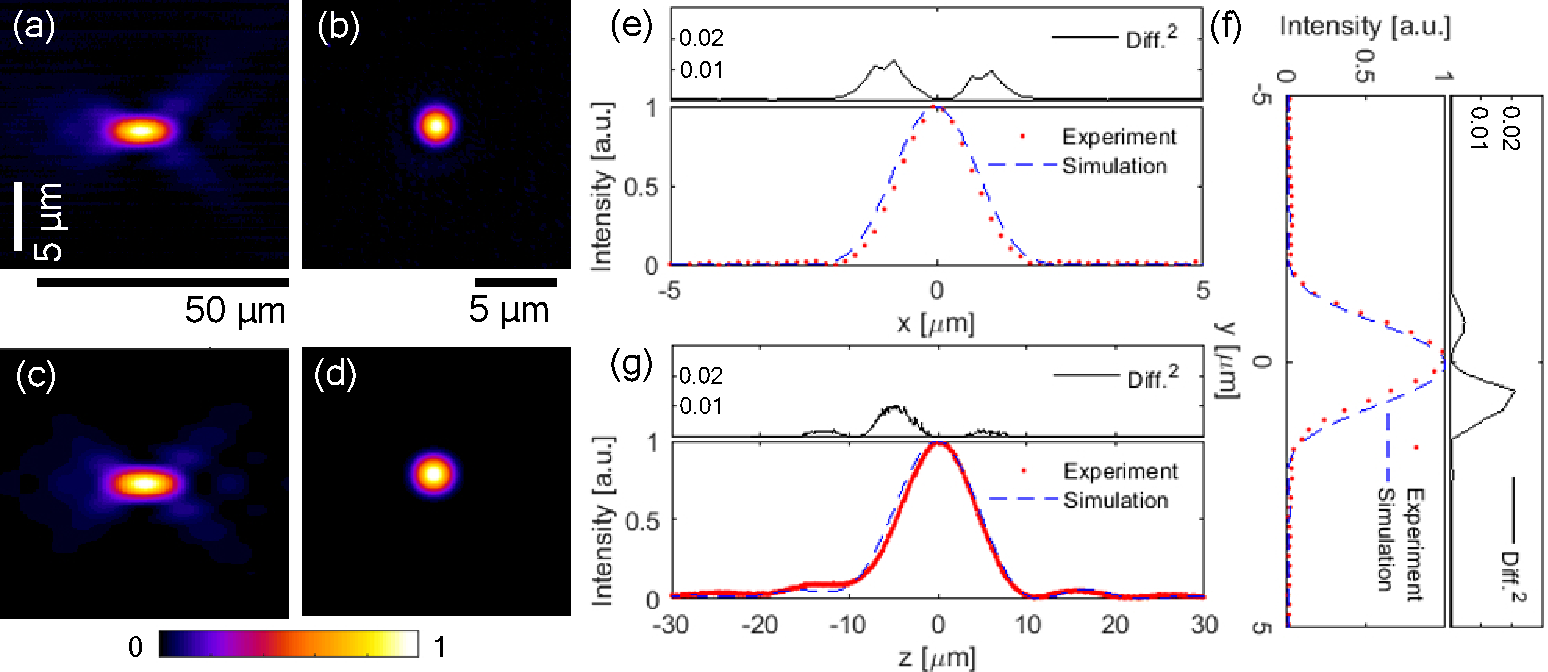
\includegraphics[width=\linewidth]{../AppOptics/figures/C240TME-C.pdf}
	\caption{Intensity distribution near the focus of a aspherical lens (C240TME-C) in air with a gaussian beam as the input. (a) Experimentally measured intensity along x-z plane; (b) experimentally measured intensity at the focal plane; (c) simulated intensity along x-z plane; (d) simulated intensity at the focal plane. And intensity profiles comparisons at the focal plane (e) along the x-axis; (f) along the y-axis. (g) Intensity profiles comparison along z-axis.}\label{fig:3b}
\end{figure}

\subsection{Exotic beams focused by objective lens in air}
The microscope objective lens are also widely used for laser beam focusing and material processing. Working in its designed wavelength, the aberration can often be corrected. In section, we chose the 20$\times$ Mitutoyo Plan Apo objective lens (NA = 0.4) as the focus lens. The central wavelength of the laser is chose as 1030-nm. And instead of using a standard Gaussian beam as the input, we chose the amplitude/phase shaped beams for the demonstration. To precisely simulate the focusing conditions, we first record the intensity profile of the exotic beam at the entrance pupil of the objectives with an array of image sensors, and then calculate the amplitude distribution by take the square root of the intensity profile. Based on those measured 'user defined' amplitude profiles and their polarization states, we can achieve the complex fields on the entrance pupil by multiplying with the engineered phase information. Finally, based on \eqref{eq:17} and \eqref{eq:23}, the fields near the focus can be calculated. These calculated intensity distributions are compared with the experimental results. 

\begin{figure}
	\centering
	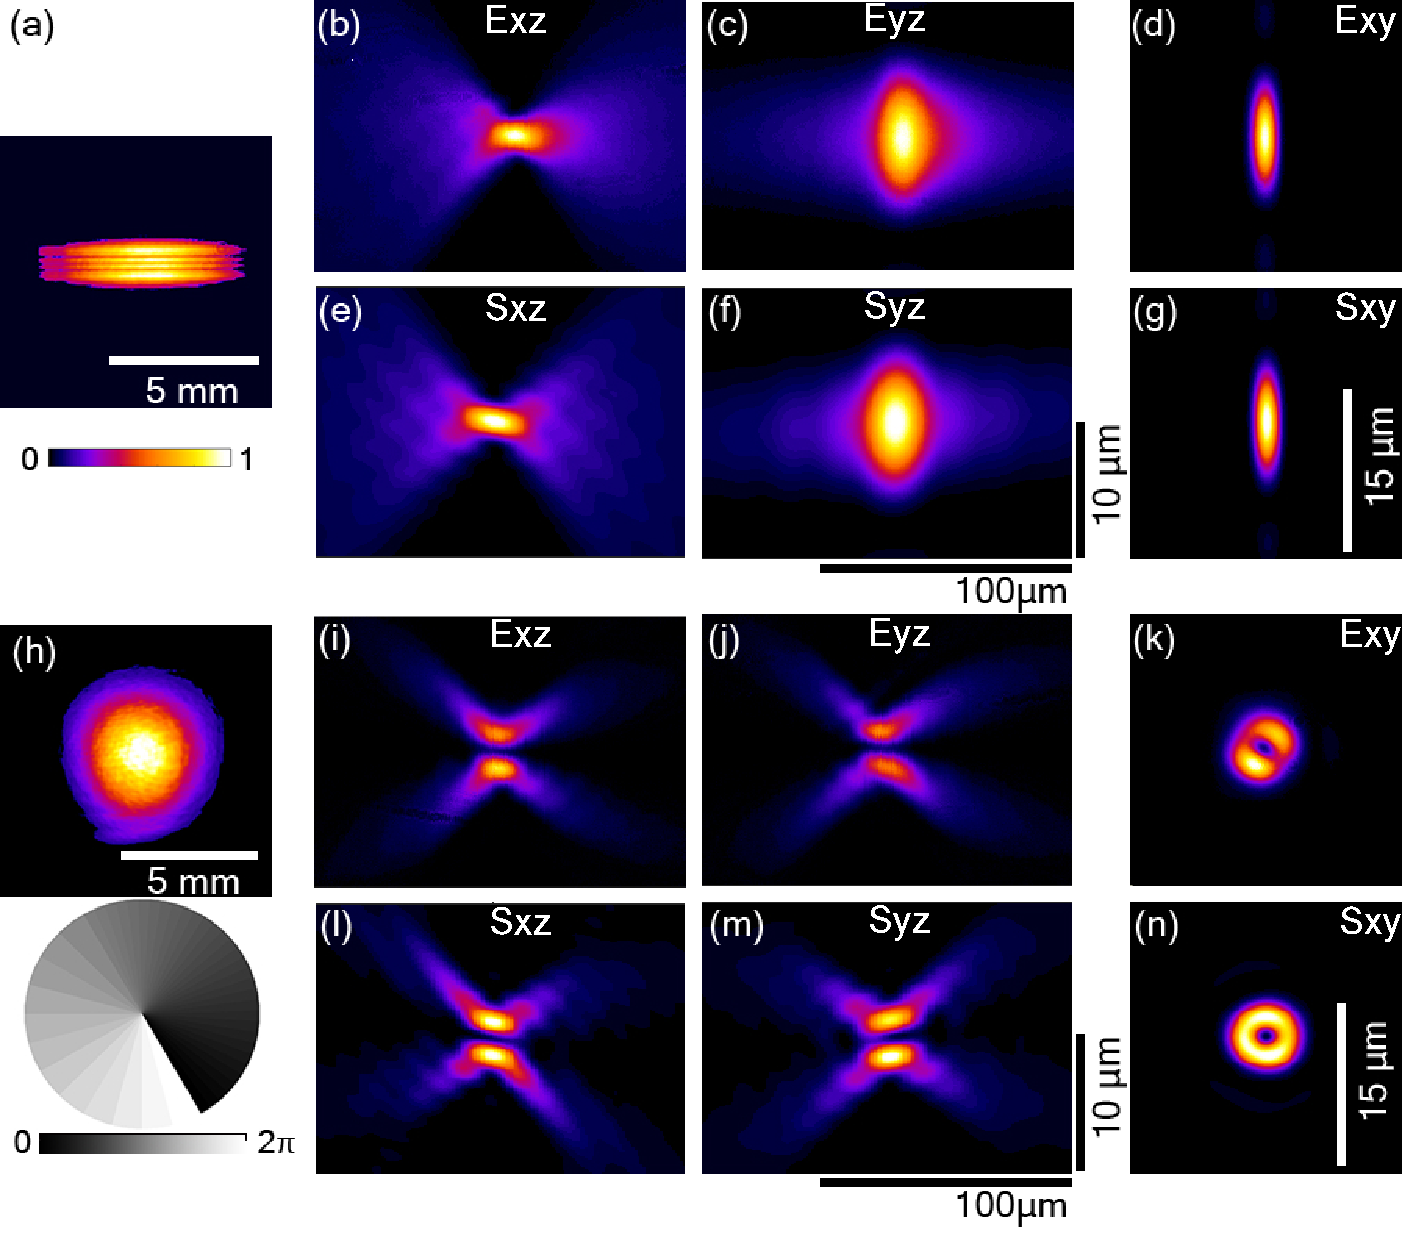
\includegraphics[width=\linewidth]{../AppOptics/figures/20xairExotic.pdf}
	\caption{Intensity distribution of the input beam at the entrence pupil, (e) a gaussian beam cutted by a slit with width of 1.38-mm. Intensity distributions near the focus, (a-b) Experimentally measured intensity along x-z and y-z plane; (c-d) simulated intensity along x-z and y-z plane; (f) experimentally measured intensity at focal x-y plane; (g) simulated intensity at focal x-y plane. }\label{fig:4}
\end{figure}

A circular cross-sectional focusing is often required for single-mode waveguides or microfluidic channels writting. Slit beam shaping is a simple technique that provides such isotropic resolution in transverse and vertical direction \cite{cheng2003control, ams2005slit}. In this section, we use the slit beam shaping as a first demonstration to prove that our methods are also applicable for the amplitude shaped beam. 

As shown in Fig.~\ref{fig:4} (a), a Gaussian beam with $1/e^2$ radius of 5.2~mm is cutted by a 1.38-mm width slit. When this linear polarized beam is focused the objective lens, the measured intensity distributions are shown in Fig.~\ref{fig:4} (b-d) and the simulated results are shown in Fig.~\ref{fig:4} (e-g). At the focal plane, as shown in Fig.~\ref{fig:4} (d), the beam wasit along x-axis is measured as 2.9~$\mu$m and along y-axis is 10.9~$\mu$m. Comparing with the simulated results shown in Fig.~\ref{fig:4} (g), the beam waists exhibit the same value. By comparing the longitudinal results (b-c) and (e-f), the presented experimental and simulated focusing features are consistent, i.e. at first the laser beam is less tightly focused in y-z plane compare to the one in x-z plane and secondly the axis of the intensity center is tilt against z-axis. These features can be explained as at first the input beam is deficient filled the entrence pupil along y-axis and overfilled along x-axis which leads a relatively low effecitve numerical aperature in y direction, and secondly the input laser beam profile is rather then a perfect gaussian distribution but exhibits some asymmetrical features. It is worth noting that the second feature is revealed in the simulation results only when it allows to use the real intensity distribution at the entrance pupil as the input. All in all, a nearly perfect match of the results empowered the two methods for investigating senarios which have more sophisticate anisotropic input beams. \hl{However, one should be careful when applying our computational method under the extremely asymmetric condition such as the line-focus microscopy (LTM), since Wolf has proposed that his Debye integral representation should be considered only beyond a critical value of the Fresnel number} \cite{wolf1981conditions}. \hl{The Fresnel number is a dimensionless number, $\mathcal{N} = a^2/\lambda f$, which reflects the relative contribution of focusing vs. diffraction effects for a given aperture radius $a$, focal length $f$, and wavelength $\lambda$. For a more rigorous approach dedicated to this specific problem, a recently research has been carefully addressed by Lou \emph{et~al.}} \cite{lou2018better}. \hl{They illustrated that when the Fresnel numbers close to unity the focus must shift backward, thus leading to astigmatic focusing when the circular symmetry of the input light is broken. In our case, the Fresnel number in y direction is as high as 41, which explains why we could not observe this backward shift in the experiment and makes our simulation results acceptable.}   

Moreover, phase shaping is also tested in this section. Over the last dacade, the helical wavefront is one of the most extensively studied complex phase shapes of light. This type of light beams have an azimuthal phase dependence of $\exp(il\theta)$, where $l$ is the topological charge. When focused, this optical vortex form a ring instead of a spot in the focal plane. The optical vortex has many innovative applications in optical tweezers \cite{padgett2011tweezers}, atom manipulation \cite{ladavac2004microoptomechanical} and material processing \cite{hnatovsky2010materials}. In this section, experimentally, we used a spiral phase plate (SPP) to discretely generate an azimuthal phase distribution of $\exp(-i1\theta)$. The topological charge is -1, and the number of discrete steps is 12. After the phase plate, it get focused the objective lens. In the simulation, to obtain the corresponding complex field as the input, we multiplied the measured amplitude distribution with a discrete spiral phase map that exhibits the same phase distribution as the one used in experiment. The measured input intensity distribution and the calculated spiral phase map are presented in Fig.~\ref{fig:4} (h).

The simulated results are shown in Fig.~\ref{fig:4} (l-n). Comparing with the experimental results (i-k), it presents the same optical vortex feature. From the longitudinal intensity distributions (i-j) and (l-m) one can see that in both cases the light waves along the propagation axis cancel each other out and the ratios of the outer and inner radius are identical. At the focal plane, as shown in Fig.~\ref{fig:4} (k) (n), this ratio is measured as 4.3 (experimental) and 4.0 (simulated). However, even in general the results achieved by the two methods are identical, one can still notice some deviations in terms of the spot ellipticity and the intensity homogeneity. Those deviations are most probably due to the imperfection of the spiral phase plate and its misalignment to the central of the beam.          

\subsection{Gaussian beam focused by objective lens in bulk of silicon}
In the previous sections, the laser beams are focused in the air. In this section, the in-bulk focus condition is chose for demonstration. When an planar interface is present, according to aberration function \eqref{eq:14}, the interface-induced aberration is a function of the focus depth, the numerical aperature and the refractive index of the bulk material. When a gaussion beam ($\lambda$: 1555-nm, waist: 5.2-mm) is focused into a 5-mm thick cuboidal crystalline silicon (c-Si) sample (n = 3.475 at 1555-nm) by an objective lens with NA of 0.65, the interface-induced aberration is prominent. Applying the same methods, we can achieve the experimental and simulated results of the longitudinal intensity distributions near the focus. When the focus depth is chose as 5-mm and the propagation direction is from the left to the right, the experimental result is presented in Fig.~\ref{fig:5} (a) and corresponding simulated result is shown in Fig.~\ref{fig:5} (c). Differed from the previous cases, the comparison shows significant deviation in terms of overall length. And the reason of this deviation is that, as the propagation measurements procedures indicated, this measured result is actually not the intensity distribution in the bulk with focal depth of 5-mm. Precisly speaking, it is the stacking of intensity profiles at the exit surface of the 5-mm sample while the focusing objective lens moved step-by-step from -1.5 to +0.5~mm refering the exit surface. To distiguish it from the real distribution in the bulk, Fig.~\ref{fig:5} (b-c) show the simulated distribution with focal depth of 4-mm and 5-mm, comparing with the experimental result, the 4-mm result has a similar overall length but the relative intensity of the right hand side 'tail' is much lower, and the 5-mm result shows a longer overall distribution length.
\begin{figure}
	\centering
	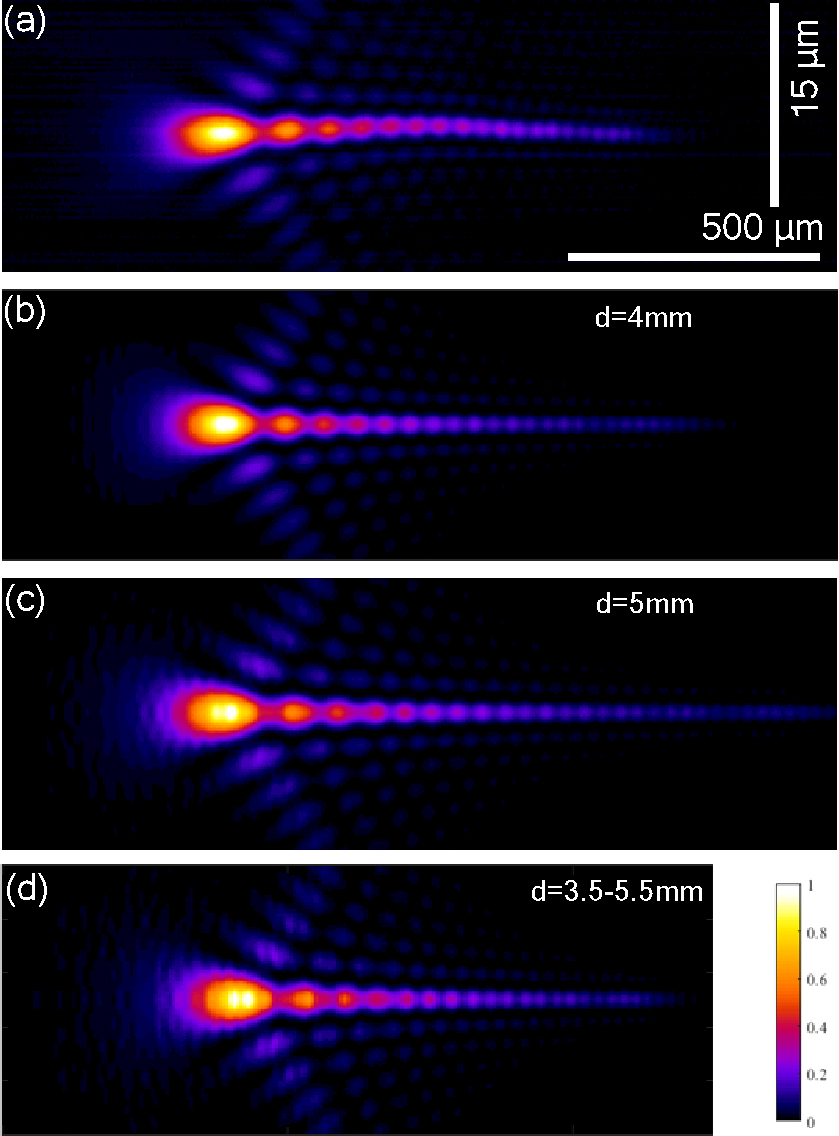
\includegraphics[width=\linewidth]{../AppOptics/figures/50xSi.pdf}
	\caption{Intensity distributions near the focus, (a) Experimentally measured intensity along x-z plane; (b-c) simulated intensity along x-z plane with focal depth of 4-mm and 5-mm; (d) simulated intensity at the exit surface of the 5-mm sample with focal depth varies from 3.5-mm to 5.5-mm.}\label{fig:5}
\end{figure}

A spontaneous question raised here is 'why not directly measure the intensity distribution in the bulk?'. However, unfortunately, experimentally it is unlikely to measure the real intensity distribution. If we fix the position of the focusing objectives and move the recording microscope, the recorded images would also affect by the depth related aberration during the step-by-step moving. The only way to avoid the artificial result is to compensate the depth related aberration after each movement. Considering we have more than two thousands steps, it is unrealistic to compensate it with any simple tools such as correction collar. However, this measured result can still help to benchmark our simulation method.

\begin{figure}
	\centering
	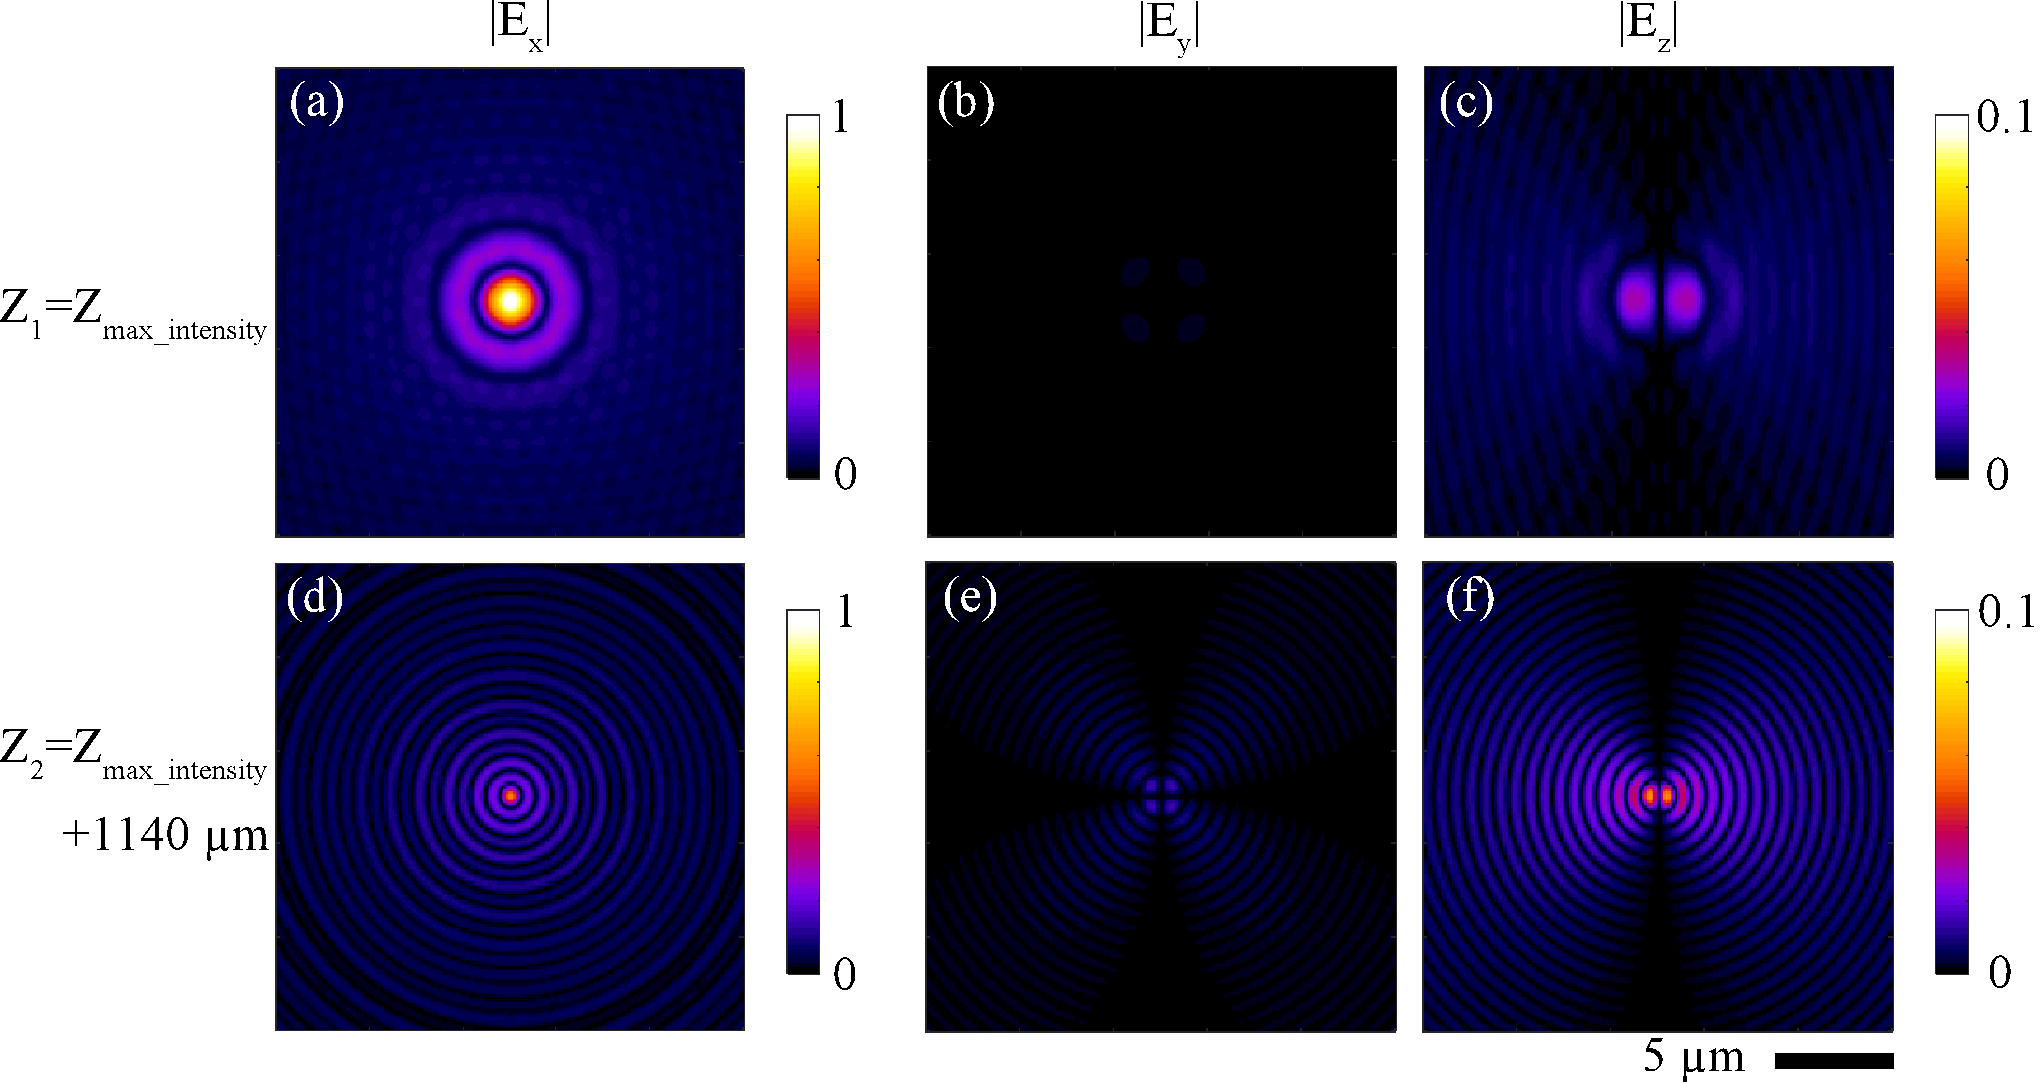
\includegraphics[width=\linewidth]{../AppOptics/figures/50xPolarization.pdf}
	\caption{Intensity distributions near the focus, (a) Experimentally measured intensity along x-z plane; (b-c) simulated intensity along x-z plane with focal depth of 4-mm and 5-mm; (d) simulated intensity at the exit surface of the 5-mm sample with focal depth varies from 3.5-mm to 5.5-mm.}\label{fig:6}
\end{figure}

In order to simulate the experimental condition, we first calculate the corresponding intensity profile at the exist surface of the 5-mm sample under different focal depths (from 3.5 to 5.5~mm). The focal depth increment stepsize is 5~$\mu$m. After the calculation, we stack the intensity profiles from the left to the right with the focus depth decrement from 5.5~mm to 3.5~mm. By taking those two steps, it simulate the image acquisition procedures of the experimental condition and the corresponding image intensity distribution is displaced in Fig.~ref{fig:5} (d). Compare to (b) and (c), it shows better similarity in terms of overall length and relative intensity along the profile to the experimental result (a).

Therefore, if a laser beam is focused into a bulk material and we want to investigate the intensity distribution over a large area of interest along the propagation direction, extra caution should be paid when any experimental methods is applied. 

Besides, since in this demonstration the numerical aperature is as high as 0.65, even the incident beam is linear polarized along x-direction, the polarization near the focus will no longer be pure x-polarized. When the focal depth is set as 5-mm, the amplitude of the three polarization components near the focal regime is displaced in Fig.~\ref{fig:6}. At the plane where maximum total intensity is located, as shown by Fig \ref{fig:6} (a-c), the maximum amplitude of the x-component is about 457 times higher than the y-component and 34 times higher than the z-component. The maximum total intensity plane is overlapped with the maximum $|E_x|$ plane, however it shifts away from the maximum $|E_y|$ or $|E_z|$ plane for about 1140~$\mu$m. The maximum $|E_y|$ and $|E_z|$ planes are overlapped, and located at the right tail of the intensity profile shown in Fig.~\ref{fig:5} (c). As shown in Fig.~\ref{fig:6} (d-f), the maximum amplitude of $|E_x|$ at this plane is about 37 and 9 times higher than the maximum amplitude of $|E_y|$ and $|E_z|$, which is much lower compare to the maximum total intensity plane. This observation indicates that, when a linear polarized laser beam is focused into a bulk material by a high NA lens, it will not only generate new polarization components near the focus, the maximum amplitude planes of each components are also shifted.
\section{Conclusion}
In this paper, we introduced two useful tools for analysing the field distribution when a laser beam is focused in air or in any cuboidal materials. A vectorial analysis model which considered the lens-induced as well as the planar interface-induced aberration, and an in-bulk propagation imaging setup with 300-nm longitudinal resolution and diffraction limited lateral resolution are presented. The theoretical method is benchmarked by the experimental reuslts, and the simulation results can also remedy the limitation of the experimental method. With these tools, people can deal with a variety of real focus conditions in which arbitrary input fields, non-aplanatic lens, and in-bulk focus might involved. As an application example in the field of laser in-bulk processing, one can use our tools to calculate the aberration free condition in which the spherical aberration is counterbalance by the planar interface-induced aberration.

In conclusion, the two tools we provided allow for accurate and efficient analysis of the focused volumetric field distribution. By sharing them to a broader community, it helps researchers and engineers to create and verify their new in-bulk processing ideas in a faster way.


%%%%%%%%%%%%%%%%%%%%%%% References %%%%%%%%%%%%%%%%%%%%%%%%%

%%%%%%%%%% If using BibTeX:
\bibliography{references}

\end{document}
